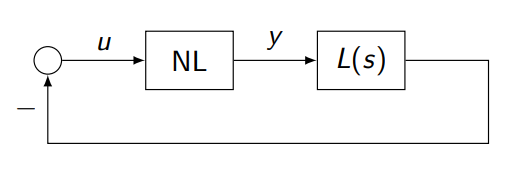
\includegraphics[width = \linewidth]{src/images/nolinearity_block_diagram.png}
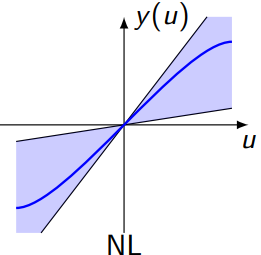
\includegraphics[width = \linewidth]{src/images/nolinearity_plot.png}
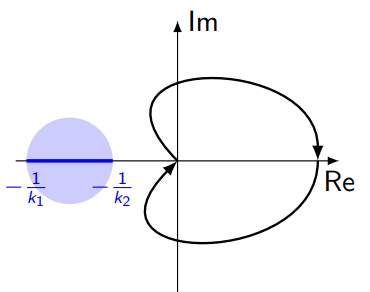
\includegraphics[width = \linewidth]{src/images/nolinearity_nyquist.png}

Nolinearity can be bounded by linear funktion of slope $k_1$ and $k_2$. Nyquist condition now applies to a circle.\\
Necessary condition: For some of the given nonlinearities, the system is stable (Nyquist plot can go through the circle)\\
Sufficient condition: For all of the given nonlinearities, the system is stable (Nyquist plot does not go through the circle)

Examples of static nonlinearities:
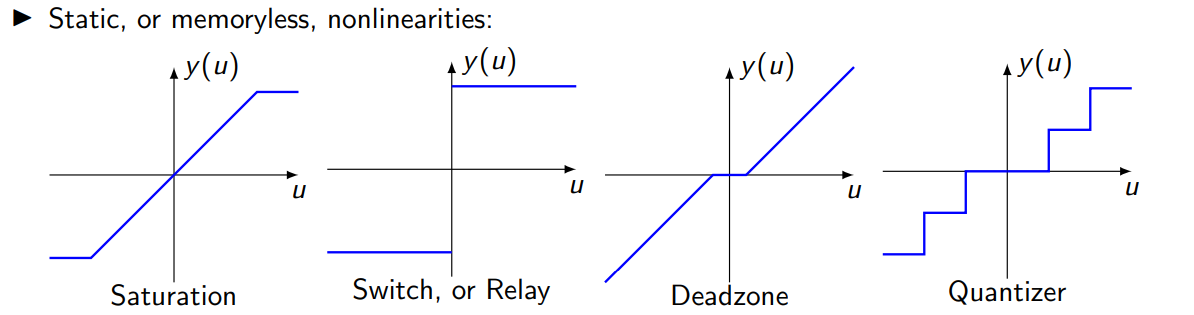
\includegraphics[width = \linewidth]{src/images/nonlinearity_example.png}

\subsection{Describing Function}
    Every Output $y(t)$ with a sinusodial input function $u(t) = A \sin(\omega t)$ can be written as a fourier series:
    \begin{align*}
        y(t) = \frac{a_0}{2} + \sum\limits_{i = 1}^{\infty}[a_i \cos(i \omega t) + b_i \sin(i \omega t)]\\
        a_i = \frac{1}{\pi} \int\limits_{-\pi}^{\pi} y(t) \cos(i \omega t) d(\omega t)\\
        b_i = \frac{1}{\pi} \int\limits_{-\pi}^{\pi} y(t) \sin(i \omega t) d(\omega t)
    \end{align*}
    For odd nonlinearity y: $a_i = 0$\\
    We are interested in the first harmonic of an odd function. Therefore 
    \begin{align*}
        y(t) \approx b_1 sin(\omega t)\\
        \text{describing function: } N(A) = \frac{b_1(A)}{A} = \frac{1}{\pi A} \int\limits_{-\pi}^{\pi} y(t) \sin(i \omega t) d(\omega t)
    \end{align*}

\subsection{approximate describing function}
    \begin{align*}
        \text{For input } u(t) = Ae^{j \omega t}\\
        y(t) \approx c_1(A, \omega) e^{j(\omega t + \phi_1(A, \omega))}\\
        N(A, \omega) = \frac{c_1(A, \omega)}{A} e^{j \phi_1(A, \omega)}
    \end{align*}

\subsection{Stability analysis of nonlinear systems}
    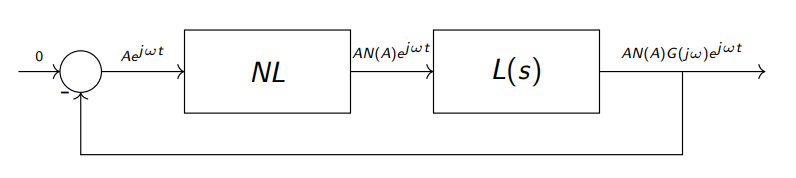
\includegraphics[width = \linewidth]{src/images/nonlinear_stability_block_diagram.png}
    \begin{align*}
        NL \cdot L(s) = \L'(A, s) \approx N(A) L(s)\\
        \text{self-sustained oscillation: }\\
        A e^{j \omega t} = A \cdot N(a) \cdot G(j \omega) e^{j \omega t}\\
        \Leftrightarrow - \frac{1}{N(A)} = G(j \omega)
    \end{align*}
    If the above equation holds, the oscillation is self sustained and so called limit cycles can arise.
    Graphically spoken, Limit cycles can occur when the nyquist plot of $- \frac{1}{N(A)}$ and $G(j \omega)$ intersect\\
    \begin{itemize}
        \item If the $-\frac{1}{N(A)}$ point is in an “unstable” region in the Nyquist plot, the amplitude of the
        oscillations will tend to increase;
        \item If the $-\frac{1}{N(A)}$ point is in a “stable” region in the Nyquist plot, the amplitude of the
        oscillations will tend to decrease;
    \end{itemize}
    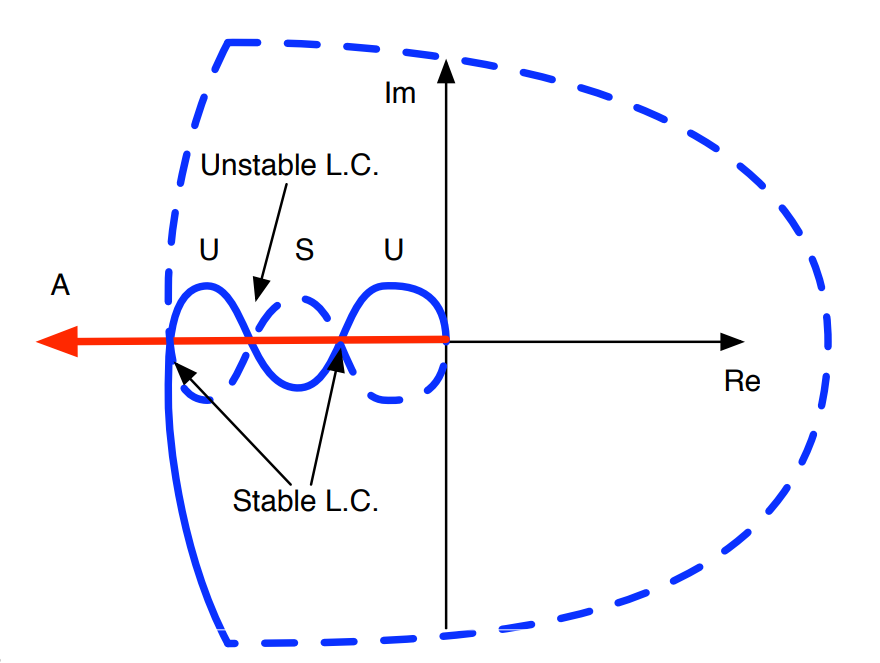
\includegraphics[width = \linewidth]{src/images/nonlinearity_stability_limit_cycles.png}